\subsection{Vereinzelung} 
\label{sec:Vereinzelung}
\textit{(ygu)} Die Umsetzung der Vereinzelung orientiert sich stark am realisierten Funktionsnachweis. Der grundlegende Aufbau wurde beibehalten. Hinzu kommen einige Erweiterungen, um die Zuverlässigkeit und die Benutzerfreundlichkeit zu steigern.

\subsubsection{Aufbau und Funktion}
Die Vereinzelung besteht aus einer Trommel (Punkt. 1 in Abbildung \ref{fig:details_vereinzelung}), worin die NemaCaps eingefüllt werden. Durch die Rotation der Lochmaske (3), welche durch einen Getriebemotor (7) umgesetzt wird, fallen die NemaCaps in die vorgesehenen Löcher . Überschüssige NemaCaps werden durch mehrere Bürsten (6) abgestreift. Sobald die vereinzelten NemaCaps bei den Schlauchkupplungen (8) angekommen sind, sollen diese durch die Schläuche zur Einsetzlokalität fallen. Alle Komponenten werden auf einer Grundplatte (4) montiert, wobei diese in ihrer Neigung verstellbar gelagert ist.
	\begin{figure}[H]
	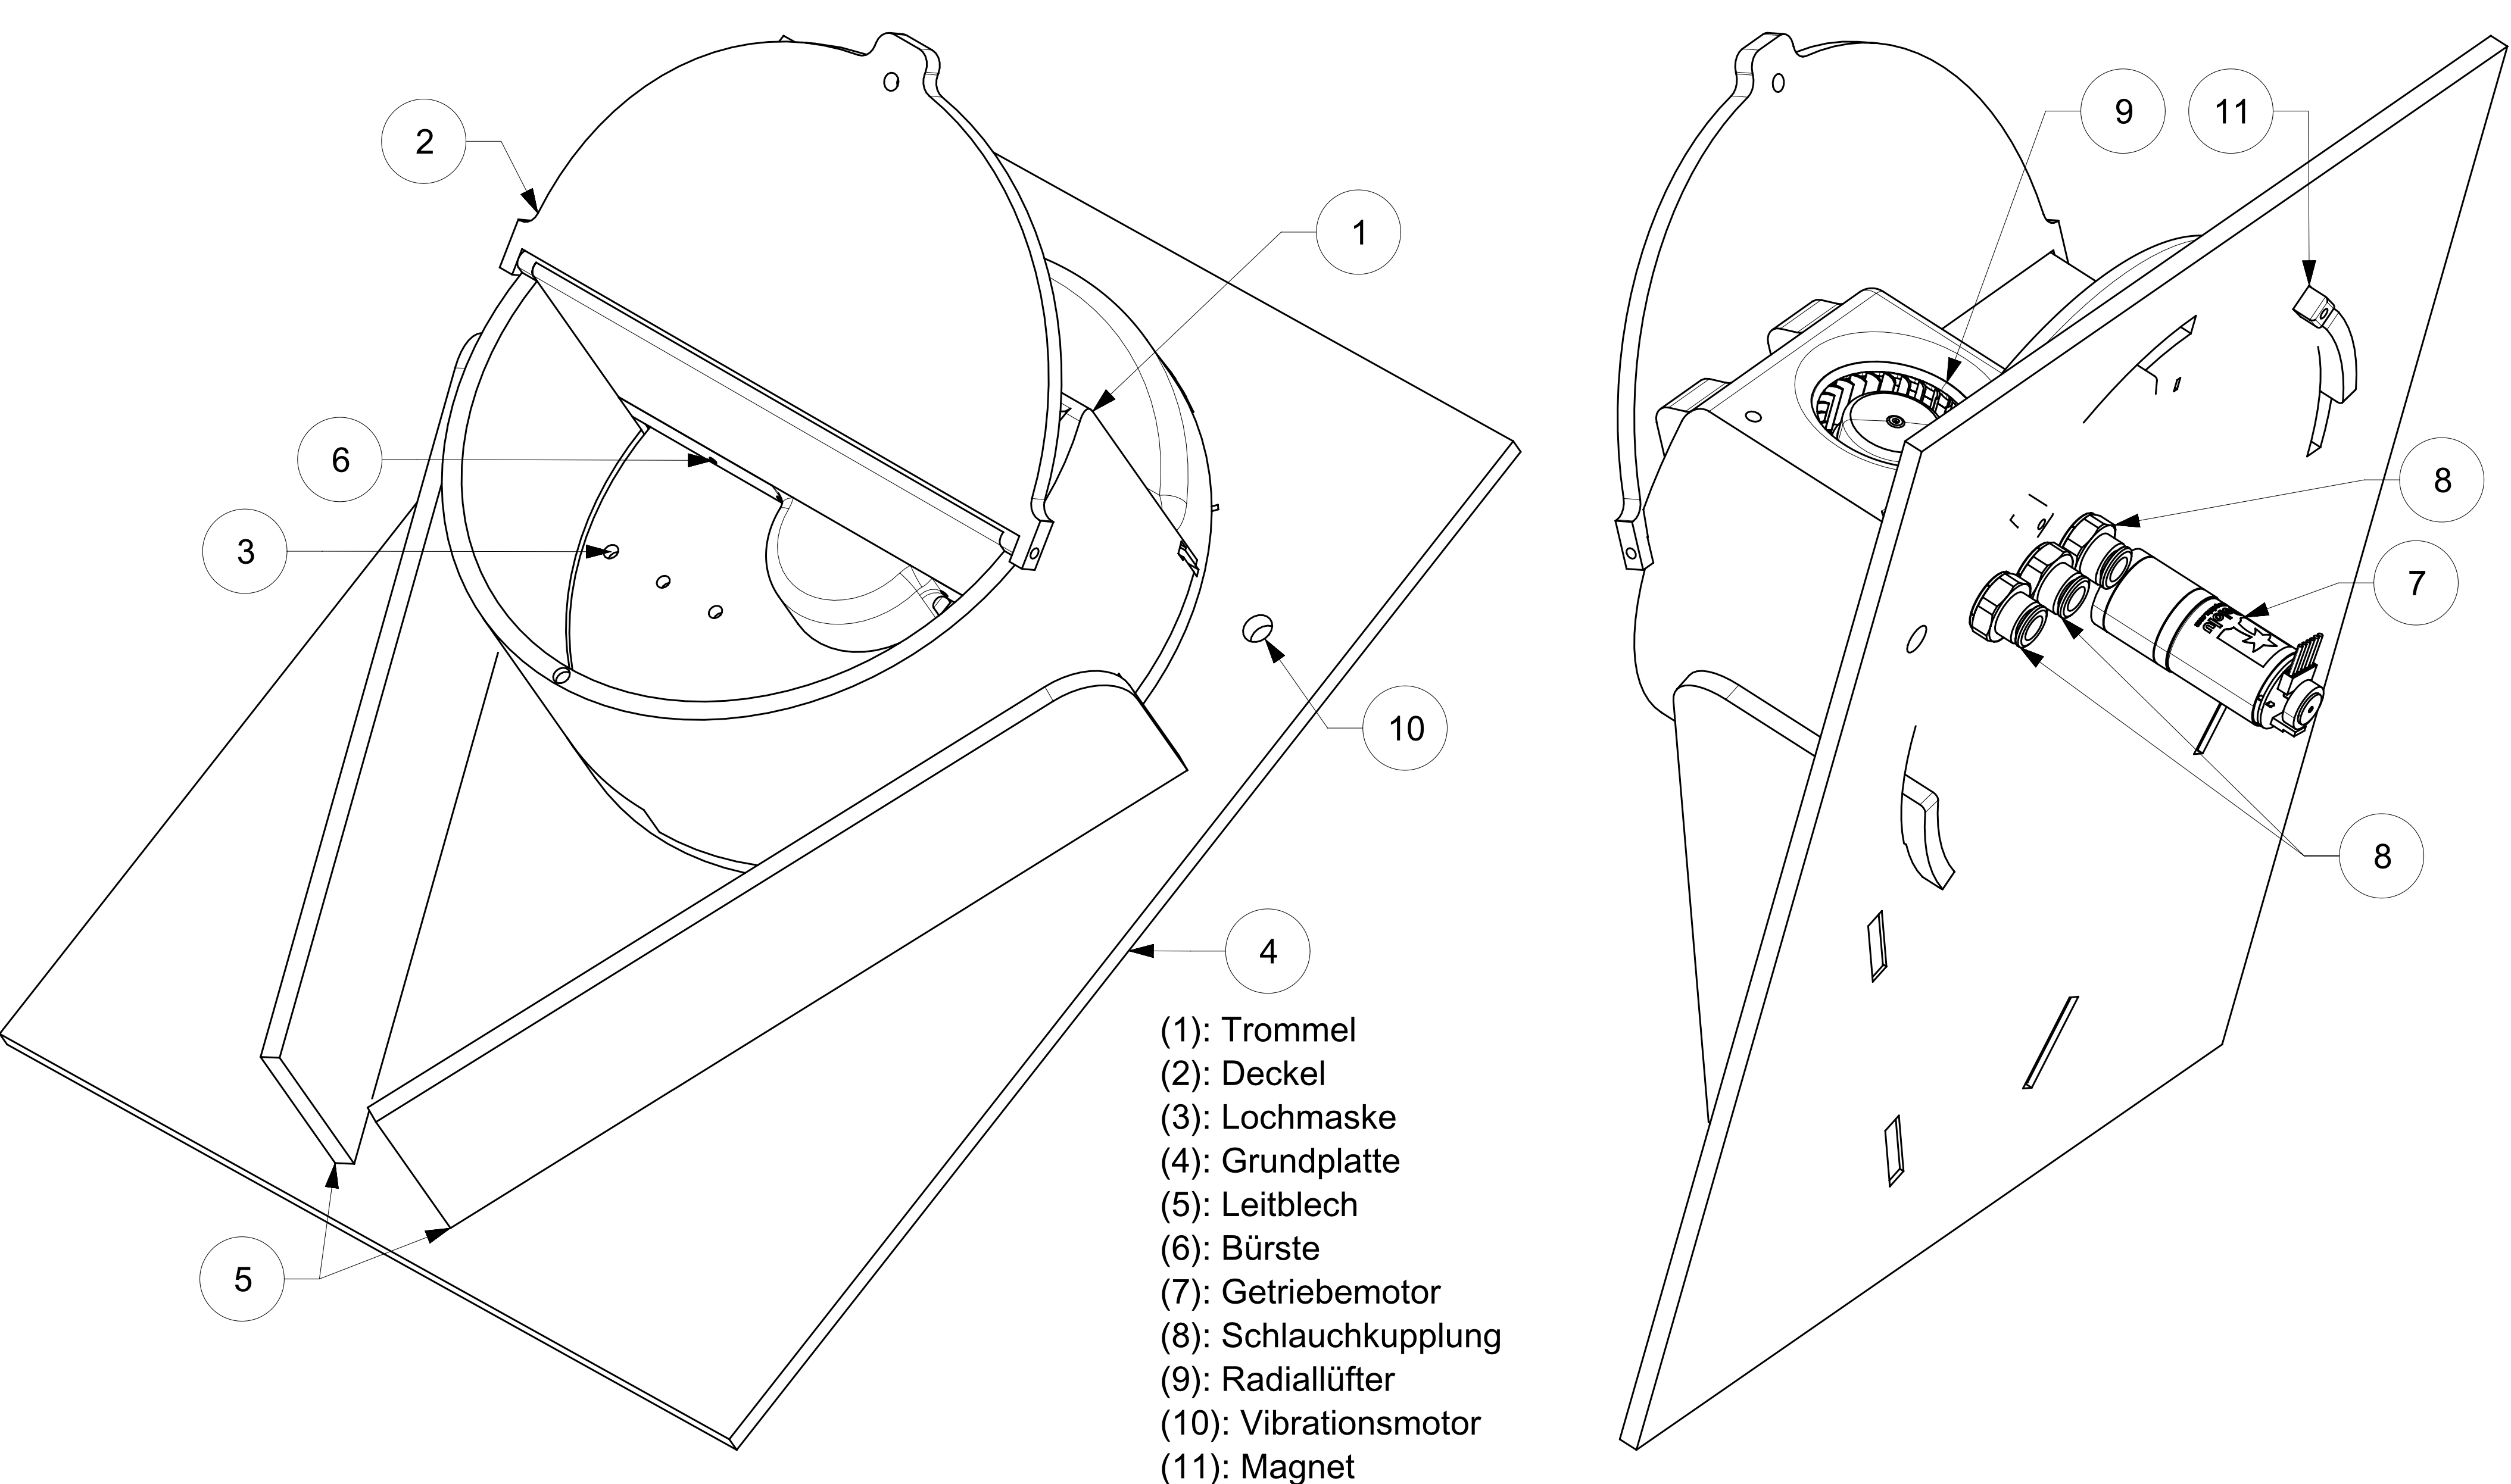
\includegraphics[scale=0.455]{Illustrationen/6-Umsetzung/details_vereinzelung.jpg}
	\caption{Detaillierte Übersicht der Vereinzelung}
	\label{fig:details_vereinzelung}
	\end{figure}

\subsubsection{Abhilfemassnahmen}
\label{abhilfe}
Der Funktionsnachweis aus Kapitel \ref{funktionsnachweis} zeigte auf, dass Komplikationen auftreten können. In erschwerten Bedingungen, wie nassem Pulver, kann das NemaCap  durch die erhöhte Adhäsion an der Lochmaske hängen bleiben. So wurde im Funktionsnachweis die Bedingung formuliert, dass eine Umsetzung dieser Funktion nur mit konkreten Abhilfemassnahmen umgesetzt werden darf, um die Zuverlässigkeit der Vereinzelung zu steigern. Diese sind:
\begin{itemize}
	\item \textbf{Vibrationsmotor:} Der Funktionsnachweis zeigte, dass durch leichtes Klopfen an der Einheit, hängengebliebene NemaCaps erfolgreich gelöst werden. Somit wird in der Nähe der Schlauchkupplungen ein Vibrationsmotor (Punkt. 10 in Abbildung \ref{fig:details_vereinzelung}) angebracht, welche die Einheit in Schwingung bringen soll. Wichtig ist die Grundplatte in einer Richtung federnd zu lagern, sodass diese tatsächlich in Schwingung geraten kann.

	
	\item \textbf{Radiallüfter:} Eine weitere Möglichkeit die NemaCaps zu lösen, bietet ein gezielter Luftstoss. Daher ist in der Trommel ein Radiallüfter (9) integriert, welcher einen Luftstrom auf die vereinzelten NemaCaps in der Lochmaske richtet. Bei Bedarf werden zusätzliche Löcher an den Schläuchen angebracht, um den Luftaustritt zu verbessern. 
	
	\item \textbf{Lochmaske:} Am Funktionsnachweis wurde ersichtlich, wie kritisch die Materialwahl sowie Fertigungsqualität der Lochmaske ist. Die formulierten Punkte zur Steigerung der Zuverlässigkeit sind im Kapitel \ref{lochmaske} erläutert.
\end{itemize}

\subsubsection{Handhabung}
Die Verwendung von frischen NemaCaps trägt zur verbesserten Zuverlässigkeit der Vereinzelung bei. Der benutzerfreundliche Wechsel von NemaCaps ist also ein wichtiges Anliegen und wird in der Konstruktion der Vereinzelung berücksichtigt. So ist die Trommel (Punkt 1 in Abb. \ref{fig:vereinzelung_entleeren}) mit einem dreifachen Bajonettverschluss (Detail C in Abb. \ref{fig:vereinzelung_entleeren} und Punkt 12 in Abb. \ref{fig:details_vereinzelung}) versehen. Die Trommel kann mit einer Drehung von 15° im Gegenuhrzeigersinn entriegelt werden (Detail A in Abb. \ref{fig:vereinzelung_entleeren}). Nun kann die Trommel entfernt werden (Detail B). Die verbleibenden NemaCaps (Detail X) rollen nun auf der Grundplatte hinunter. Geleitet durch zwei Leitbleche (5) fallen diese in Richtung Detail Y, wo man diese in einem Behälter sammeln kann. Auch verfügt die Trommel über einen Deckel (2), welcher durch zwei angebrachte Magnete sicher verschlossen wird.
	\begin{figure}[H]
	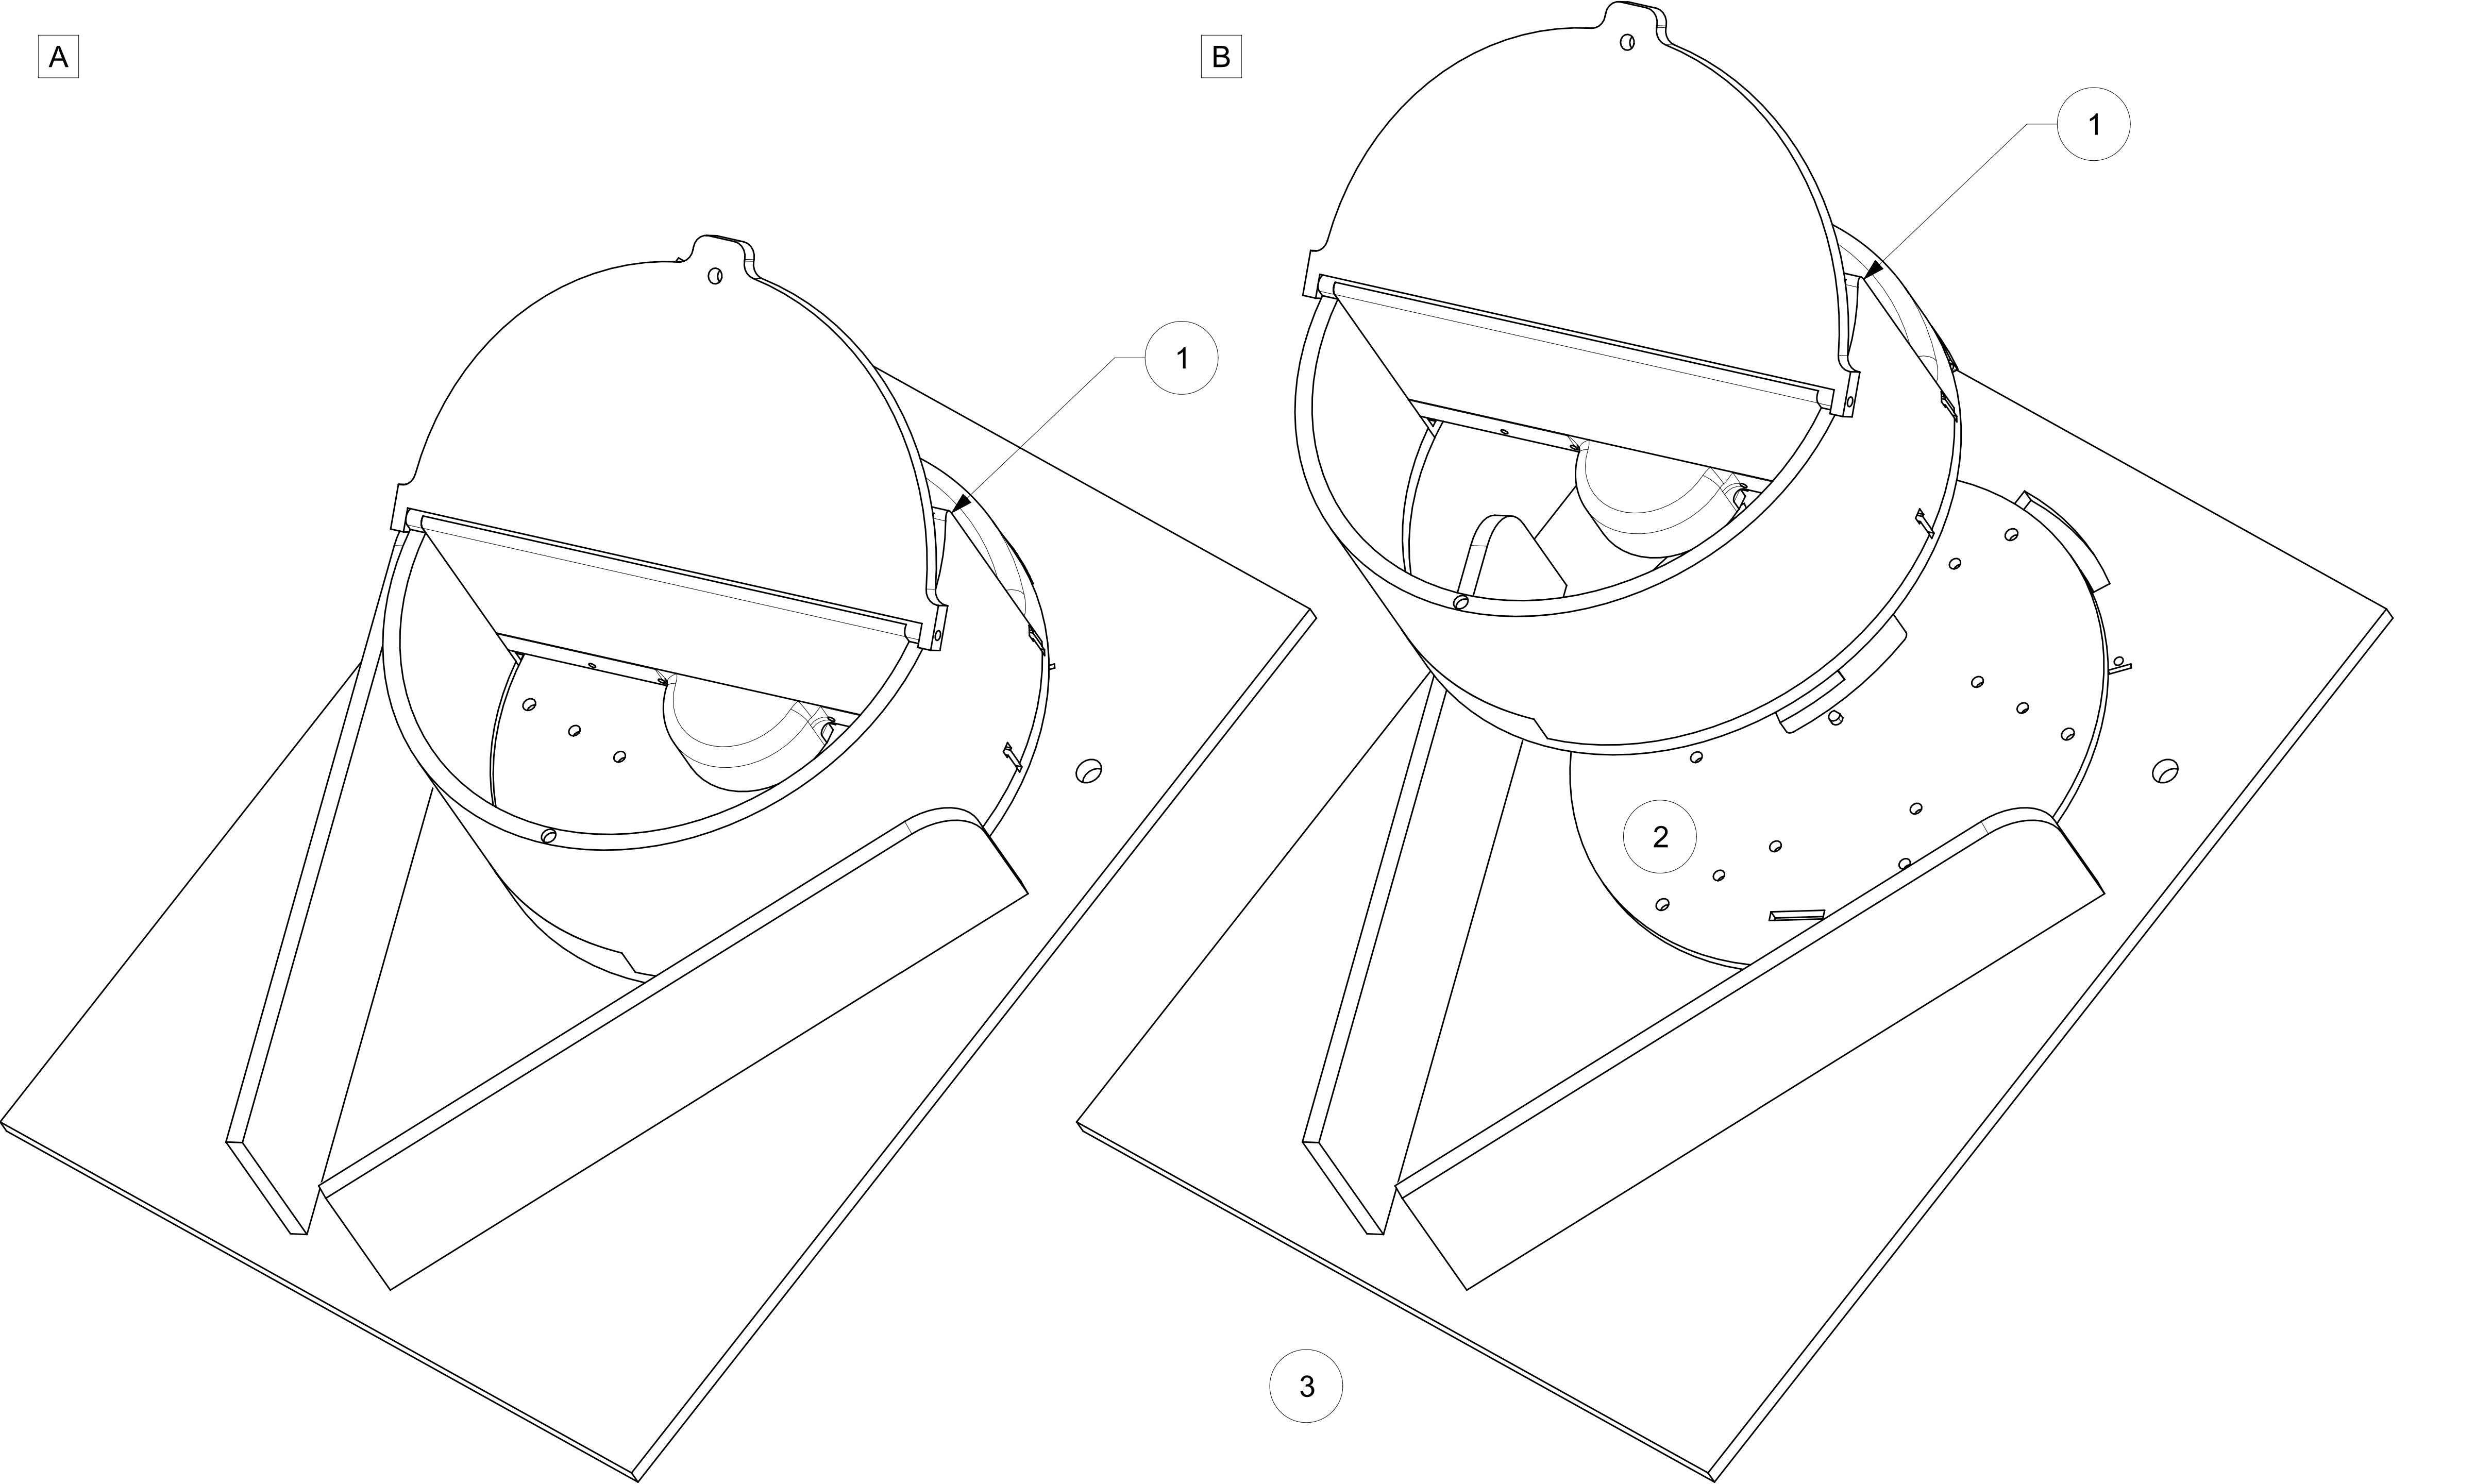
\includegraphics[scale=0.42]{Illustrationen/6-Umsetzung/vereinzelung_entleeren.jpg}
	\caption{Entleerung der Trommel}
	\label{fig:vereinzelung_entleeren}
	\end{figure}
\subsubsection{Lochmaske}
\label{lochmaske}
Der Funktionsnachweis hat gezeigt, dass das Scheitern der Vereinzelung meist durch das Hängenbleiben der NemaCaps an der Lochmaske verursacht wird. Die Zuverlässigkeit dieser Funktion hängt direkt von den Eigenschaften der Lochmaske ab. Die Materialwahl sowie Fertigungsqualität von diesem Teil ist entscheidend. 
\newline
Folgende Massnahmen werden umgesetzt:
\begin{itemize}
	\item \textbf{Materialwahl:} Die Wahl des passenden Materials mit der geringsten Adhäsion wurde mittels praktischen Tests am 26.4.2017 durchgeführt. Dabei wurden gängige laserbare Materialien (Aluminium, Plexiglas und MDF) miteinander verglichen. Die Tests zeigen, dass Aluminium die geringste Adhäsion gegenüber von NemaCaps aufweist, gefolgt von Plexiglas. Mit MDF wurde die grösste Adhäsion festgestellt, was sich durch die erhöhte Pulveraufnahme und die rauhere Oberfläche erklären lässt. 
	Die höchste Zufriedenstellung wird mit Aluminium erreicht, wobei die Reibung zwischen Lochmaske und Grundplatte noch nicht berücksichtigt ist. Bei zu hoher Reibung kann auf Plexiglas ausgewichen werden.
	
	\item \textbf{Fertigungsqualität:} Die Tests vom 26.4.2017 zeigten auch, dass die Rauheit der Oberfläche relevant ist. Je feiner die Oberfläche der Bohrung (Punkt 13 in Abbildung \ref{fig:detail_lochmaske}), desto geringer das Risiko, dass NemaCaps hängenbleiben. Folglich werden diese Löcher nach der Bohrung zusätzlich mit einer Reibale (\textbf{H7?}) ausgerieben. Der ideale Durchmesser D1 muss während der Inbetriebnahme durch zielgerichtetes Ausprobieren erörtert werden.
	
\end{itemize}
Desweiteren ist die Lochmaske mit zwei Langlöchern (14) ausgestattet. Diese werden zur Einpassung von Dauermagneten verwendet, welche zur Positionsbestimmung der Lochmaske dienen. Der Abstand B in Abbildung \ref{fig:detail_lochmaske} ist gegeben durch die Grösse der Schlauchkupplungen (Punkt 8 in Abb. \ref{fig:details_vereinzelung}) und kann dadurch nicht verkleinert werden \cite{camozzi2}.
	\begin{figure}[H]
	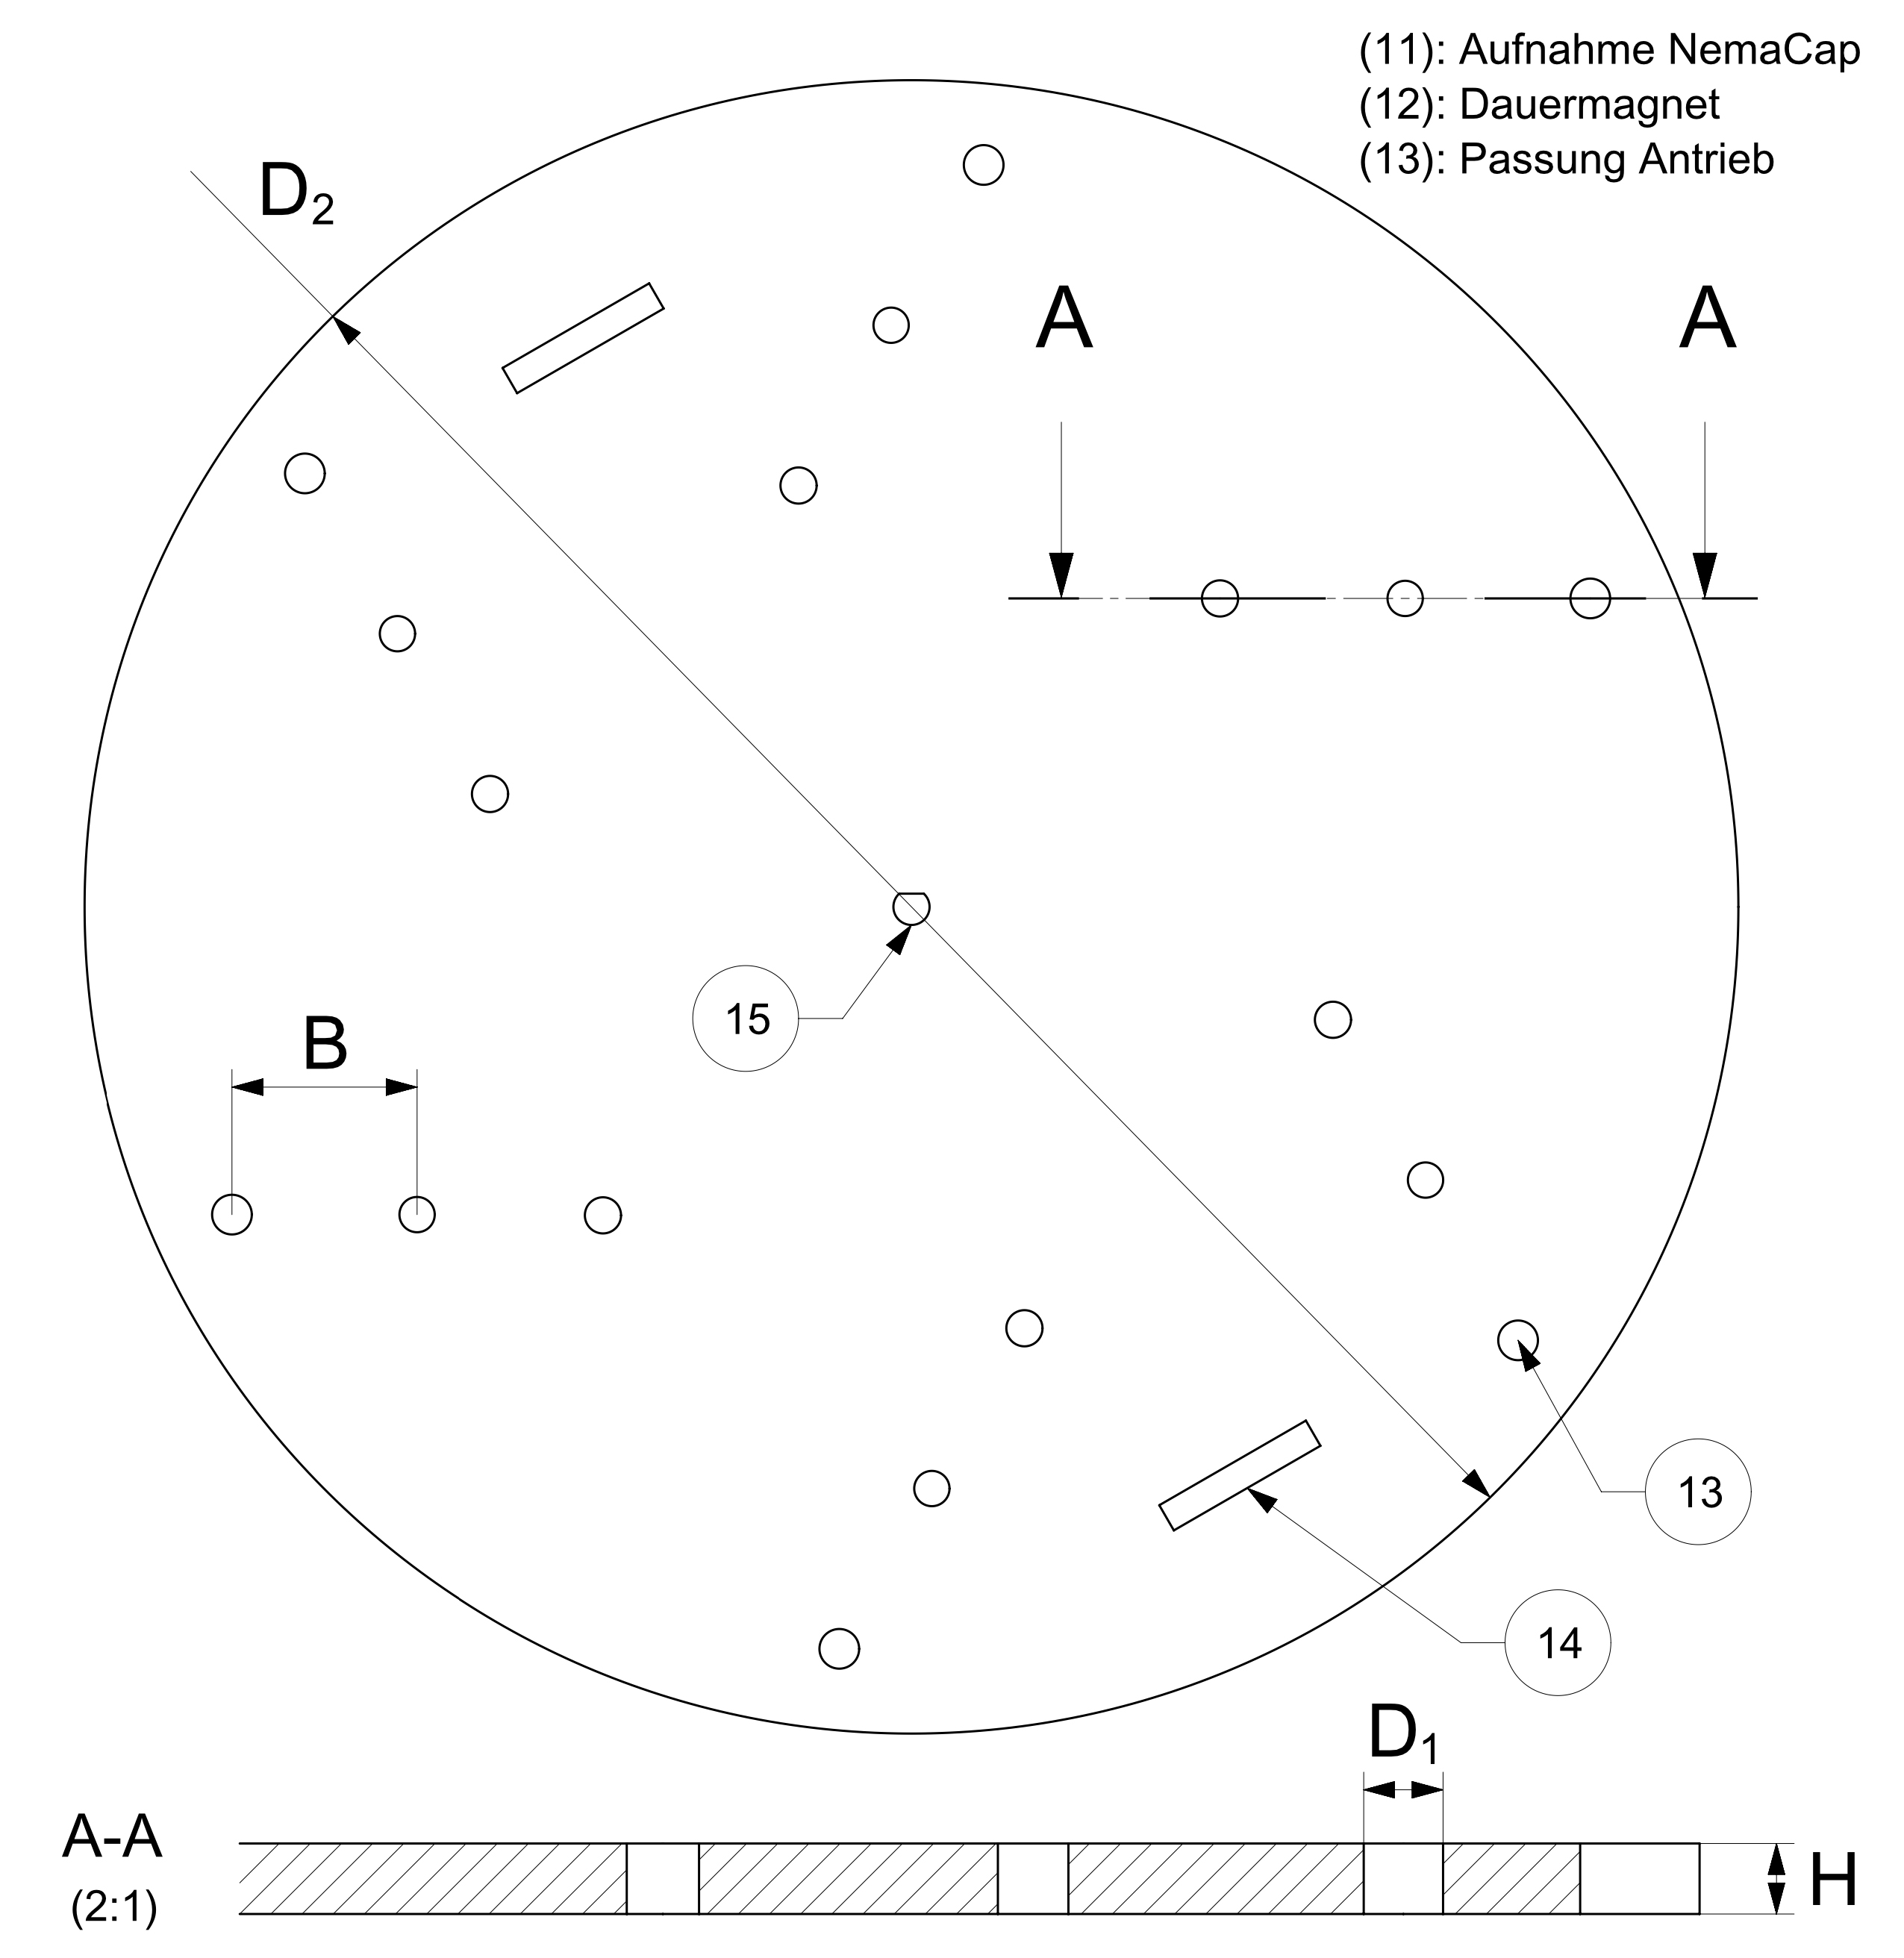
\includegraphics[scale=0.65]{Illustrationen/6-Umsetzung/detail_lochmaske.jpg}
	\caption{Grundriss der Lochmaske mit Schnitt}
	\label{fig:detail_lochmaske}
	\end{figure}

\subsubsection{Prozessablauf}
\textit{(pro)} Die Vereinzelung benötigt einen drehmomentstarken Antrieb um eine flüssige Funktion zu gewährleisten. Dafür wird ein DC Getriebemotor von Pololu mit einer Getriebeübersetzung von 99:1 verwendet. Die Spezifikationen, sowie die Begründung für die Wahl dieser Antriebstechnik sind in Kapitel \ref{kap:Evaluation_der_Komponenten} erläutert.
\\ Um die Lochmaske präzise positionieren zu können, kommen zwei Sensorik Systeme zum Einsatz. Ein Hall Sensor zur absoluten Bestimmung der Position der Lochmaske, sowie der Quadratur Encoder des Motors zur Bestimmung des zurückgelegten Winkels relativ zur gemessenen Position. Es wird der digitale Hall Sensor SS441A von Honeywell verwendet (siehe Abb. \ref{fig:SS441A}). Das Bauteil kann mit einer Spannung von 3.8V bis 30V betrieben werden. Die typische Stromaufnahme beläuft sich dabei bei einer Spannung von 5V auf 6.5mA. Der Hall Sensor reagiert auf den Südpol des verwendeten Stabmagneten und löst bei Raumtemperatur bei einem magnetischen Feld von 55G aus.

\begin{figure}[H]
	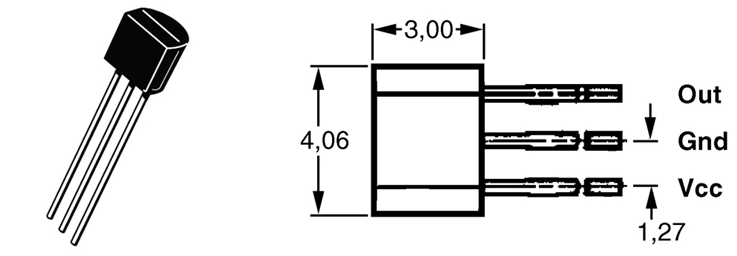
\includegraphics[width=0.9\textwidth]{Illustrationen/6-Umsetzung/Hall_Sensor.png}
	\caption{SS441A, digitaler Hall Sensor \protect\cite{SS441A}}
	\label{fig:SS441A}
\end{figure}

Das System initialisiert sich nach einem Neustart einmalig und ist dann für den Betrieb bereit. Der ganze Prozess der Vereinzelung ist in Abb. \ref{fig:Ansteuerung_Vereinzelung} illustriert.  Der Prozess wurde dabei in vier Etappen unterteilt welche mit den Ziffern 1... 4 nummeriert sind.

\begin{figure}[H]
	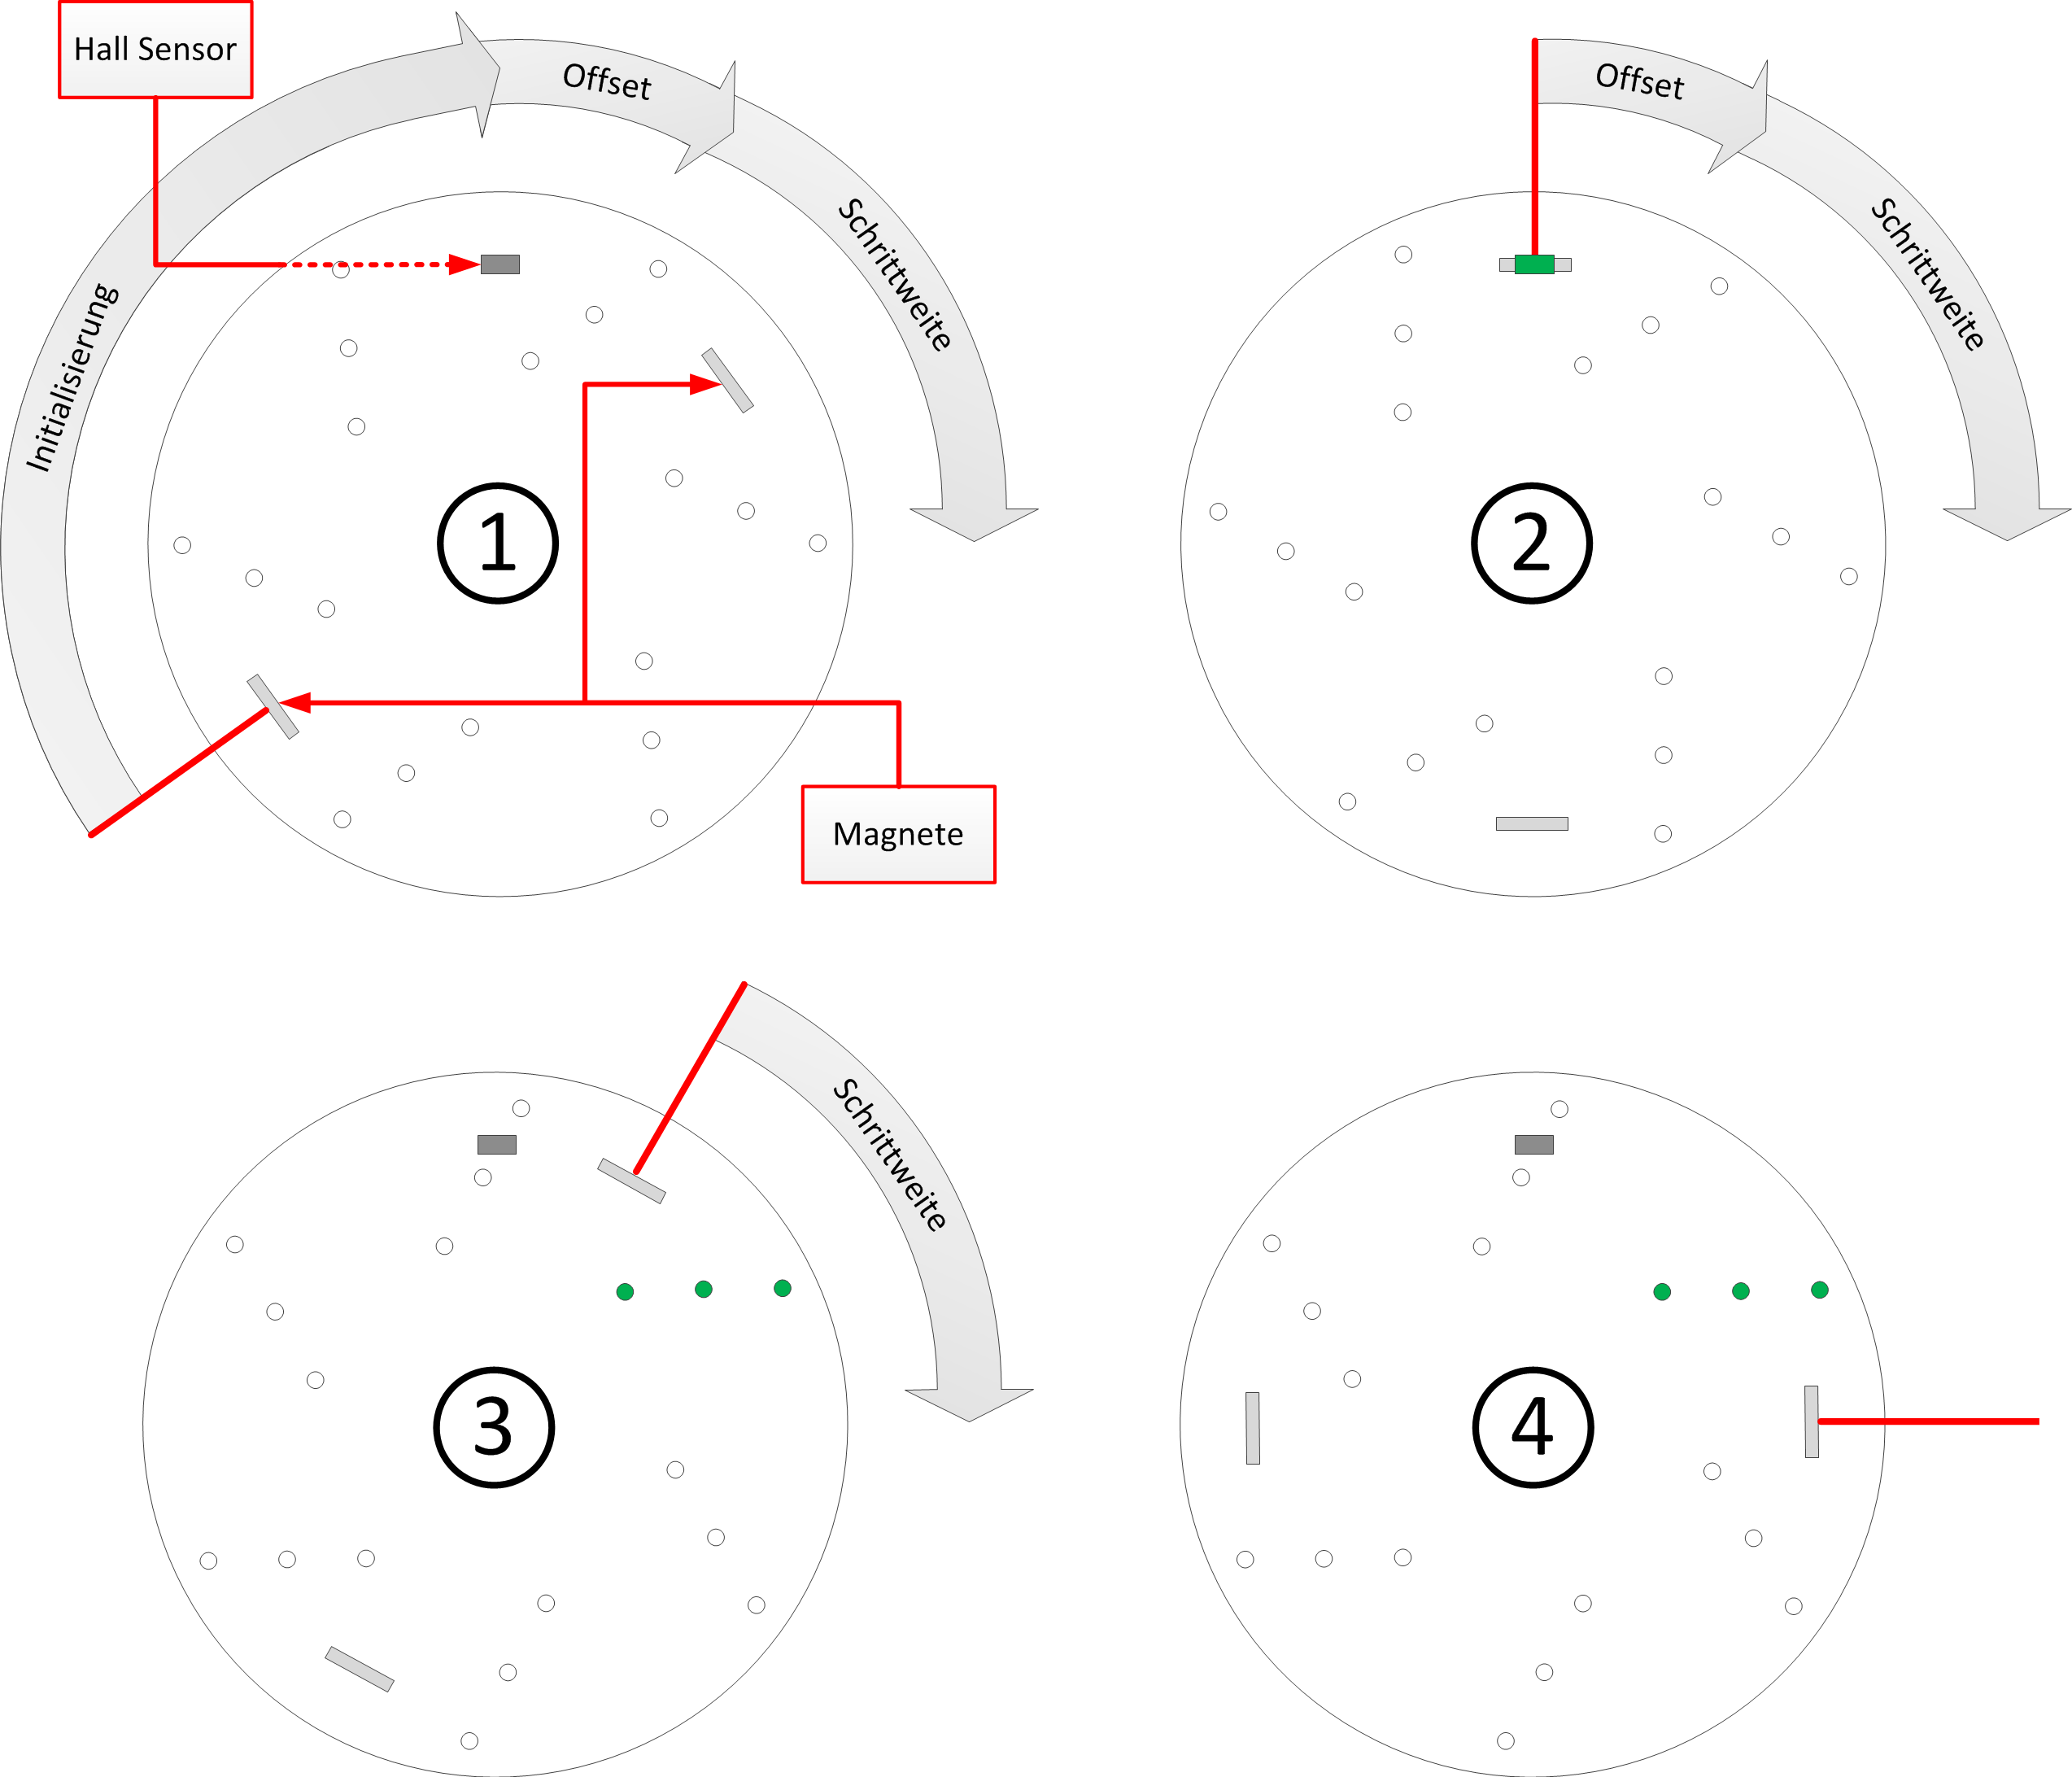
\includegraphics[width=0.9\textwidth]{Illustrationen/6-Umsetzung/Prozessablauf_Vereinzelung.png}
	\caption{Prozessablauf der Vereinzelung}
	\label{fig:Ansteuerung_Vereinzelung}
\end{figure}

Im folgenden Abschnitt werden die vier Etappen erläutert:

\begin{enumerate}
	\item Die Lochmaske wird solange gedreht bis einer der beiden Permanentmagnete, welche sich mit der Lochmaske drehen, den Hall Sensor erreichen. Der Hall Sensor ist fest hinter der Lochmaske montiert.
 	\item Zu diesem Zeitpunkt hat ein Magnet den Hall Sensor erreicht. Die Lochmaske wird eine definierte Anzahl Encoder Counts (Offset) weiter gedreht, bis die Löcher der Lochmasken übereinstimmen.
 	\item Das System ist nun initialisiert und bereit für den Betrieb. In dieser Etappe der Vereinzelung stimmen die Löcher der Lochmaske überein und die Nemacaps fallen durch die Lochmaske. 
	\item Die Nemacaps werden nun durch drehen der Lochmaske mit einer definierten Anzahl Encoder Counts (Schrittweite) repetitiv ausgelöst.
\end{enumerate}

Auch nach der Initialisierungsphase wird jedes mal wenn ein Magnet den Hall Sensor erreicht, die Position der Lochmaske neu ermittelt. Dadurch wird eine mögliche Ungenauigkeit durch aufaddieren der Fehler in der Schrittweite vermieden. Ausserdem wird dadurch der Fehler durch mögliche Impulsverluste minimiert. Die Parametrisierung des Prozessablaufs wird im Kapitel Inbetriebnahme (\ref{sec:Inbetriebnahme_Vereinzelung}) behandelt. 